% We are thrilled to announce the launch of the groundbreaking ByteBoost Cybertraining Program. ByteBoost is driven by the imperative to enhance researchers' proficiency and productivity when navigating cutting-edge, specialized computing technologies. We hope to empower researchers to make the best computing choices in the ever-changing landscape of computational technology. This initiative will focus on supporting researchers using the technologies of three NSF computing testbeds - Ookami, Neocortex and ACES.

% Program Objectives:
% Facilitate Seamless Research: Elevate the ease and productivity of researchers working with cutting-edge computing technology.
% Community Growth: Foster a well-informed community of computational researchers adept at handling the newest technologies and porting applications.
% Optimal Testbed Usage: Ensure the proper and efficient utilization of testbeds, a critical component in the recent surge of data-enabled science and engineering.
% Target Audience:
% Early career-researchers (graduate students, postdoctoral associates, and Assistant Professors) from all fields of computationally inclined research

% Submission Guidelines
% Submission must include the following
% CV (1 page) including the applicant's previous computing experiences, skills, and field of science
% Abstract (1 page) - Prospective participants are required to submit an abstract outlining the specific topic they intend to explore as a fundamental part of their application for consideration in this call for participation.
\noindent
\textit{\textbf{Foundations for Agent-based Evolution Simulation on Emerging HPC Accelerators.}}
\hfill
{\scriptsize M.A. Moreno, \texttt{morenoma@umich.edu}}

M.A. Moreno, \texttt{morenoma@umich.edu}
\end{center}
\vspace{-2ex}
\section{Introduction}
Evolutionary processes underlie key questions in public health, medicine, and natural resources management.
In conjunction with benchtop experiments and observational studies, \textbf{mathematical and computational models} play a key role in \textbf{understanding evolutionary processes} underpinning critical problems like epidemiology, antibiotic resistance, cancer biology, and conservation biology.
Emerging High-Performance Computing (HPC) hardware like the \textbf{Cerebras Wafer-Scale Engine (WSE)} will enable detailed modeling of \textbf{key cross-scale evolutionary phenomena}, such as transitions of individuality (e.g., multicellularity) and evo-epidemiological tradeoffs between pathogens' within-host dynamics and between-host transmissibility \cite{goldsby2020major,schreiber2021evolutionary}.

\section{Objectives}

The proposed workshop project will create foundational \textbf{algorithms and kernel implementations in Cerebras Software Language (CSL)} necessary to harness emerging HPC hardware accelerators for agent-based evolution simulation.
Developed simulation will investigate how \textbf{population structure} and \textbf{rare mutational events} influence \textbf{selective sweep frequency} within very large populations.
Among other application areas, sweep dynamics are pivotal in epidemiology to understanding how new pathogen strains emerge and establish within host populations \cite{markov2023evolution}.

\section{Methods}

To succeed as a tool for scientific research, simulation must be sufficiently observable.
In the case of evolutionary simulation, \textbf{phylogenetic history} (i.e., ancestry trees) is key to assessing the mode and tempo of evolution.

\begin{wrapfigure}{R}{2in}
% \begin{minipage}{3in}
\vspace{-3ex}
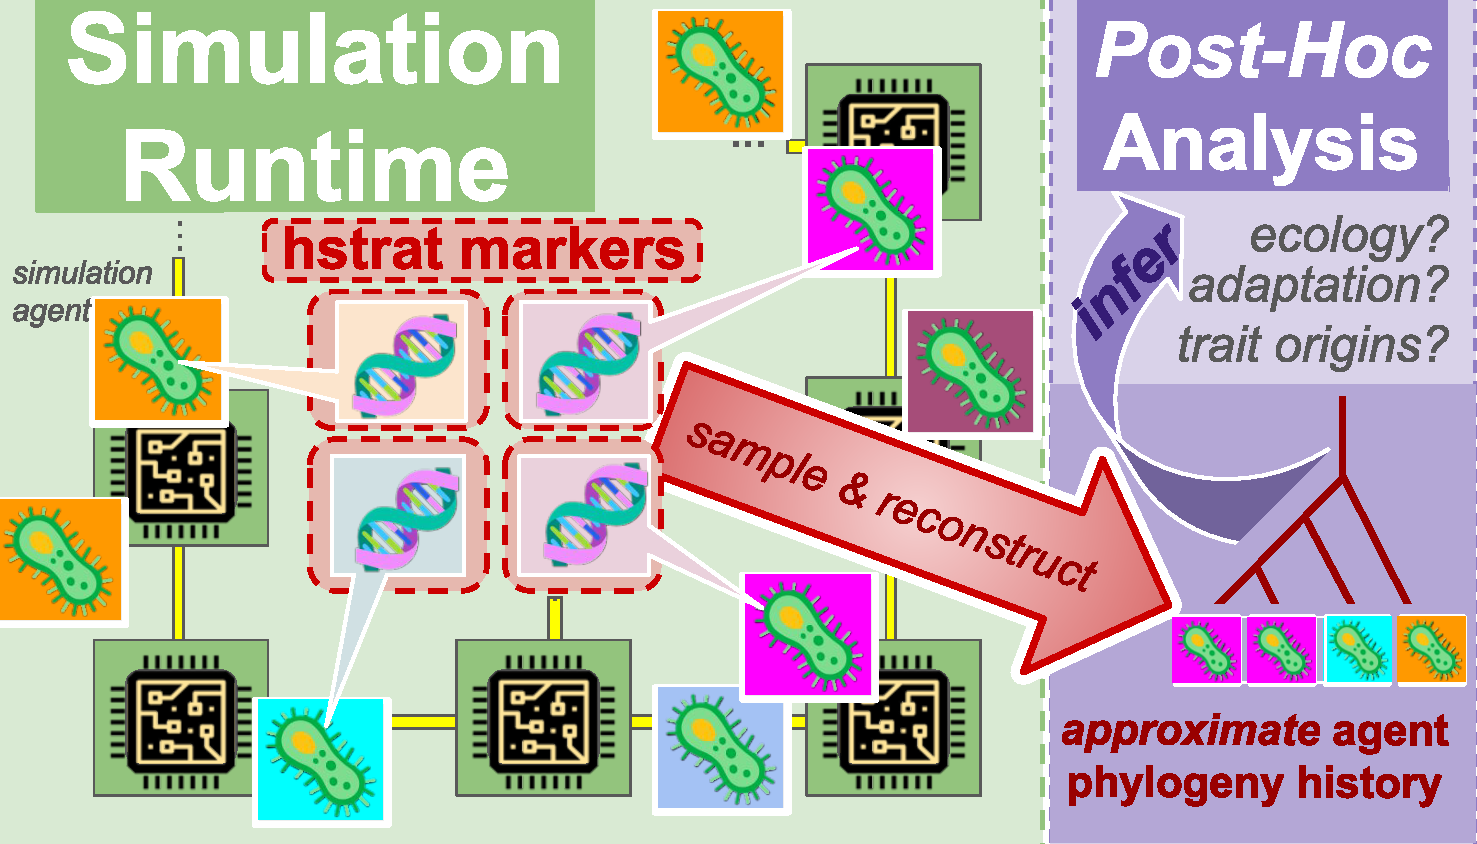
\includegraphics[width=2in]{img/runtime-posthoc-schematic.pdf}
% \end{minipage}%
% \begin{minipage}{2in}
\vspace{-5ex}
\caption{\footnotesize
Evolution simulation with reconstruction-based lineage analysis.}
\label{fig:runtime-posthoc-schematic}
\vspace{-2ex}
% \end{minipage}
\end{wrapfigure}


Proposed work builds on recently-introduced \textbf{\textit{hereditary stratigraphy} (HStrat) methods} designed to enable \textbf{extraction of evolutionary history decentralized, many-processor simulations} \cite{moreno2022hstrat}.
These methods mark population members with a special annotation akin to noncoding DNA, inherited by each consecutive generation.
After simulation ends, HStrat markers facilitate fast and accurate \textbf{reconstruction of phylogenetic history}.
This procedure, summarized in Figure \ref{fig:runtime-posthoc-schematic}, analogizes use of DNA sequence data to infer phylogenies of natural systems.
Unlike direct lineage tracking, \textbf}HStrat methods scale gracefully} to long-running multiprocess simulation \cite{moreno2024analysis}.
Markers can be as small as 96 bits.

TODO need transition

Simulation will use an \textbf{island-model algorithm} to harness HPC accelerator processing power.
This approach instantiates separate agent subpopulations per processor, with agents occasionally migrated between subpopulations.
Global population structure results from rates of agent migration and the pattern of connectivity between islands.

A simple agent model suffices for proposed work, with agent traits abstracted to a floating point ``fitness'' value encoded directly in agent genomes.
Fitness landscape properties can be tuned through choice of mutation operator.
For instance, increased probability for large fitness losses would simulate a rugged landscape.

\section{Proposed Work}

Workshop activities will build on recent \textbf{prototype implementation} of HStrat-enabled island model evolutionary simulation in CSL using the v1.0.0 Cerebras SDK, available via GitHub at \texttt{\href{https://hopth.ru/cl}{hopth.ru/cl}}.
Several engineering problems suited to workshop scope remain unresolved:
\begin{enumerate}
\item \textbf{Agent migration between distant processing elements}.
This capability enables manipulation of population structure via island capability as an experimental variable.
Possible strategies include stochastic forwarding or more structured wavelet routing schemes.
Ideally, will take advantage of as much of the routing intrinsics as possible in order to avoid making hops at each intermediate step and consuming compute cycles there.

\item \textbf{On-the-fly device-to-host genome sampling.}
Recording evolutionary intermediates over simulation runtime can help characterize evolutionary history, akin to a ``fossil record.''
This problem requires routing agent information to the periphery of the wafer and onto the host on a rolling basis.
Data export traffic will need to be balanced with agent migration, also occurring during simulation runtime.
\end{enumerate}

\section{Outcomes}

Workshop activities will combine engineering/coding with may also want to ask hypothesis driven questions.
Technical validations will precede work assessing the frequency of sweeps with different migration dynamics and mutational dynamics.

In order to assess implementations to technical problems identified above,
We will benchmark runtime cost/slowdown and assess compute capability usage.
We will benchmark the scalability of developed code by running benchmarks at different sizes of things.
We will validate migration and sampling using per-PE counters for send/receive actions and dummy genomes with fixed annotations of their origin PE identity.

Our kernel implementation will allow investigation of how population structure and rare mutational events influence selective sweep frequency within very large populations.
We will prepare an appropriate baseline treatment and assess the rate of sweeps with fat-tailed mutational distributions, strong purifying selection (high proportions of negative selection), and less spatial structure due to stronger migration rates.
and use phylogenetic reconstructions to

TODO


% will catalyze research.
% Progress on this front
% How to , to directly create modules during the workshop that can be shared.
% If there aren’t established protocols, the workshop environment would be a great place to discuss these issues.


% What is the structural relationship between individual-level phylogenies and species-level phylogenies?
% Do they respond in the same way to evolutionary conditions like selection pressure, ecology, and spatial structure?

TODO add bolding

% Project work will focus on the Cererbras WSE platform.
